% WhiteWall Studios — Design System Sheet (Phone Version)
% Compile with: xelatex design-sheet-phone.tex
% Optimized for iPhone display (9:19.5 aspect ratio, ~75mm x 163mm)
\documentclass[8pt]{article}

\usepackage[paperwidth=75mm,paperheight=163mm,margin=2.5mm,top=2mm,bottom=1.5mm]{geometry}
\usepackage{fontspec}
\usepackage{xcolor}
\usepackage{tikz}
\usepackage{graphicx}
\usepackage{enumitem}
\usepackage{parskip}
\usepackage{microtype}
\hyphenpenalty=10000
\exhyphenpenalty=10000

\pagestyle{empty}
\setlength{\parindent}{0pt}
\setlength{\parskip}{0.5pt}

% ── Colors ──────────────────────────────────────────────────────
\definecolor{wwsBlack}{HTML}{000000}
\definecolor{wwsDark}{HTML}{383838}
\definecolor{wwsLight}{HTML}{F4F4F2}
\definecolor{wwsGray}{HTML}{E0E0E0}
\definecolor{wwsAccent}{HTML}{FCD518}
\definecolor{wwsTaylors}{HTML}{C4A882}
\definecolor{wwsPowders}{HTML}{8BA7B8}

% ── Fonts ───────────────────────────────────────────────────────
\setmainfont{CormorantGaramond}[
  Path=fonts/,
  Extension=.ttf,
  UprightFont=*,
  UprightFeatures={RawFeature={+axis={wght=400}}},
]

\newfontfamily\cormorantlight{CormorantGaramond}[
  Path=fonts/,
  Extension=.ttf,
  UprightFont=*,
  UprightFeatures={RawFeature={+axis={wght=300}}},
]

\newfontfamily\cormorantsemibold{CormorantGaramond}[
  Path=fonts/,
  Extension=.ttf,
  UprightFont=*,
  UprightFeatures={RawFeature={+axis={wght=600}}},
]

\newfontfamily\interfont{Inter}[
  Path=fonts/,
  Extension=.ttf,
  UprightFont=*,
  UprightFeatures={RawFeature={+axis={wght=400}}},
]

\newfontfamily\interlight{Inter}[
  Path=fonts/,
  Extension=.ttf,
  UprightFont=*,
  UprightFeatures={RawFeature={+axis={wght=300}}},
]

\newfontfamily\intermedium{Inter}[
  Path=fonts/,
  Extension=.ttf,
  UprightFont=*,
  UprightFeatures={RawFeature={+axis={wght=500}}},
]

\newfontfamily\intersemibold{Inter}[
  Path=fonts/,
  Extension=.ttf,
  UprightFont=*,
  UprightFeatures={RawFeature={+axis={wght=600}}},
]

\newfontfamily\interbold{Inter}[
  Path=fonts/,
  Extension=.ttf,
  UprightFont=*,
  UprightFeatures={RawFeature={+axis={wght=700}}},
]

% ── Section styling ─────────────────────────────────────────────
\newcommand{\sheetsection}[1]{%
  \vspace{1.5pt}%
  {\interfont\fontsize{5}{6.5}\selectfont\addfontfeatures{RawFeature={+axis={wght=600}}}\color{wwsDark}\MakeUppercase{#1}}%
  \par\vspace{0pt}%
  {\color{wwsGray}\rule{\linewidth}{0.3pt}}%
  \par\vspace{1pt}%
}

% ── Tag command ─────────────────────────────────────────────────
\newcommand{\tag}[2][wwsGray]{%
  \tikz[baseline=(tag.base)]{%
    \node[fill=#1!20, rounded corners=1.5pt, inner xsep=2.5pt, inner ysep=1pt] (tag)
      {\interfont\fontsize{4.5}{5.5}\selectfont #2};%
  }%
}

\begin{document}

% ════════════════════════════════════════════════════════════════
% HEADER
% ════════════════════════════════════════════════════════════════
\begin{minipage}[c]{0.42\linewidth}
  \raisebox{-2pt}{
\includegraphics[height=14pt]{wws-logo.png}}%
\end{minipage}%
\hfill
\begin{minipage}[c]{0.53\linewidth}
  \raggedleft
  {\interlight\fontsize{9}{10}\selectfont Design System}\\[0pt]
  {\interfont\fontsize{4}{5}\selectfont\color{wwsDark} March 2026}
\end{minipage}

\vspace{1.5pt}
{\color{wwsBlack}\rule{\linewidth}{0.5pt}}

% ════════════════════════════════════════════════════════════════
% COLOR PALETTE
% ════════════════════════════════════════════════════════════════
\sheetsection{Color Palette}

\begin{center}
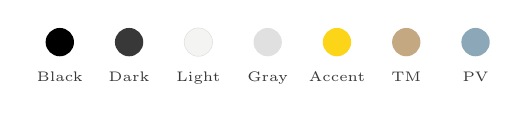
\begin{tikzpicture}
  \def\swatchspacing{0.88}
  \def\swatchradius{0.18}
  \foreach \name/\col [count=\i from 0] in {
    Black/wwsBlack,
    Dark/wwsDark,
    Light/wwsLight,
    Gray/wwsGray,
    Accent/wwsAccent,
    {TM}/wwsTaylors,
    {PV}/wwsPowders%
  }{
    \pgfmathsetmacro{\xpos}{\i * \swatchspacing}
    \ifnum\i=2
      \fill[\col] (\xpos,0) circle (\swatchradius);
      \draw[wwsGray, line width=0.2pt] (\xpos,0) circle (\swatchradius);
    \else
      \fill[\col] (\xpos,0) circle (\swatchradius);
    \fi
    \node[below, font=\interfont\fontsize{3.5}{4.5}\selectfont, text=wwsDark] at (\xpos,-0.26) {\name};
  }
\end{tikzpicture}
\end{center}

% ════════════════════════════════════════════════════════════════
% TYPOGRAPHY
% ════════════════════════════════════════════════════════════════
\sheetsection{Typography}

{\fontsize{10}{11}\selectfont\cormorantlight Cormorant Garamond}\enspace
{\interfont\fontsize{4}{5}\selectfont\color{wwsDark!60} Headings / Display}\\[0.5pt]
{\cormorantlight\fontsize{6.5}{8}\selectfont Light 300} \enspace
{\fontsize{6.5}{8}\selectfont Regular 400} \enspace
{\cormorantsemibold\fontsize{6.5}{8}\selectfont SemiBold 600}

\vspace{1pt}
{\interfont\fontsize{8}{9.5}\selectfont\addfontfeatures{RawFeature={+axis={wght=300}}} Inter}\enspace
{\interfont\fontsize{4}{5}\selectfont\color{wwsDark!60} Body / UI / Nav}\\[0.5pt]
{\interlight\fontsize{5.5}{7}\selectfont Lt 300} \enspace
{\interfont\fontsize{5.5}{7}\selectfont Reg 400} \enspace
{\intermedium\fontsize{5.5}{7}\selectfont Med 500} \enspace
{\intersemibold\fontsize{5.5}{7}\selectfont Semi 600}

% ════════════════════════════════════════════════════════════════
% LOCATION IDENTITY
% ════════════════════════════════════════════════════════════════
\sheetsection{Location Identity}

% Taylor's Mill panel

\begin{tikzpicture}
  \fill[wwsLight] (0,0) rectangle (\linewidth,1.05cm);
  \fill[wwsTaylors] (0,0.88cm) rectangle (\linewidth,1.05cm);
  \fill[wwsTaylors] (0.2cm,0.65cm) circle (1.5pt);
  \node[right, font=\cormorantsemibold\fontsize{7}{8.5}\selectfont, text=wwsBlack]
    at (0.32cm,0.65cm) {Taylor's Mill};
  \node[right, font=\interfont\fontsize{4}{5}\selectfont, text=wwsDark]
    at (0.2cm,0.4cm) {The Original Natural Light Studio};
  \node[right] at (0.12cm,0.13cm) {%
    \tag[wwsTaylors]{Portraits}\enspace
    \tag[wwsTaylors]{Branding}\enspace
    \tag[wwsTaylors]{Intimate Events}%
  };
\end{tikzpicture}

\vspace{1pt}

% Powdersville panel

\begin{tikzpicture}
  \fill[wwsLight] (0,0) rectangle (\linewidth,1.05cm);
  \fill[wwsPowders] (0,0.88cm) rectangle (\linewidth,1.05cm);
  \fill[wwsPowders] (0.2cm,0.65cm) circle (1.5pt);
  \node[right, font=\cormorantsemibold\fontsize{7}{8.5}\selectfont, text=wwsBlack]
    at (0.32cm,0.65cm) {Powdersville};
  \node[right, font=\interfont\fontsize{4}{5}\selectfont, text=wwsDark]
    at (0.2cm,0.4cm) {The Flagship Studio \& Event Space};
  \node[right] at (0.12cm,0.13cm) {%
    \tag[wwsPowders]{Weddings}\enspace
    \tag[wwsPowders]{Commercial}\enspace
    \tag[wwsPowders]{Large Events}%
  };
\end{tikzpicture}

% ════════════════════════════════════════════════════════════════
% DESIGN PRINCIPLES
% ════════════════════════════════════════════════════════════════
\sheetsection{Design Principles}

\newcommand{\principle}[2]{%
  {\intersemibold\fontsize{4.5}{5.5}\selectfont #1}\enspace
  {\interfont\fontsize{4.5}{5.5}\selectfont\color{wwsDark} #2}\par\vspace{0.5pt}%
}

\principle{Photography First}{Imagery leads, UI recedes.}
\principle{Location-Aware}{Nav adapts color per studio.}
\principle{Warm vs.\ Cool}{TM = gold; PV = blue. Never mix.}
\principle{Generous Space}{Whitespace is intentional.}
\principle{Content First}{No gratuitous animations.}

% ════════════════════════════════════════════════════════════════
% UI PATTERNS
% ════════════════════════════════════════════════════════════════
\sheetsection{UI Patterns}

{\intersemibold\fontsize{4.5}{5.5}\selectfont Buttons}\par\vspace{1pt}

\begin{tikzpicture}
  \draw[wwsBlack, line width=0.4pt, rounded corners=1.5pt] (0,0) rectangle (1.5cm,0.34cm);
  \node[font=\interfont\fontsize{4}{5}\selectfont] at (0.75cm,0.17cm) {View Gallery};
  \fill[wwsBlack, rounded corners=1.5pt] (1.7cm,0) rectangle (3.2cm,0.34cm);
  \node[font=\interfont\fontsize{4}{5}\selectfont, text=white] at (2.45cm,0.17cm) {Book Now};
  \fill[wwsAccent, rounded corners=1.5pt] (3.4cm,0) rectangle (4.9cm,0.34cm);
  \node[font=\intersemibold\fontsize{4}{5}\selectfont, text=wwsBlack] at (4.15cm,0.17cm) {Get Started};
\end{tikzpicture}

\vspace{1.5pt}
{\intersemibold\fontsize{4.5}{5.5}\selectfont Cards}\enspace
{\interfont\fontsize{4}{5}\selectfont\color{wwsDark} Flat on \texttt{\#F4F4F2}, no shadows, 1px border, 3\kern0.5pt:\kern0.5pt{}2 or 16\kern0.5pt:\kern0.5pt{}9}

\vspace{1pt}
{\intersemibold\fontsize{4.5}{5.5}\selectfont Nav}\enspace
{\interfont\fontsize{4}{5}\selectfont\color{wwsDark} Fixed top, white bg, logo left, links right, hamburger on mobile}

\vspace{2pt}
{\color{wwsGray}\rule{\linewidth}{0.3pt}}
{\interfont\fontsize{3.5}{4.5}\selectfont\color{wwsDark!50} WhiteWall Studios \enspace\textbar\enspace v1.0 \enspace\textbar\enspace March 2026}

\end{document}
